% Self-contained research-development manuscript.
% Build: pdflatex Machine_Markets_Research_Paper.tex (run twice).
% No external bibliography, figures, data, or shell escape is required.
% The Python listing in Appendix B reproduces the numerical algebra checks.
% Author identity was not supplied for this manuscript; no affiliation is implied.
\documentclass[11pt,a4paper]{article}
\usepackage[T1]{fontenc}
\usepackage[utf8]{inputenc}
\usepackage{lmodern}
\usepackage[margin=1in]{geometry}
\usepackage{amsmath,amssymb,amsthm,mathtools,bm}
\usepackage{microtype,booktabs,tabularx,longtable,array}
\usepackage{enumitem,xcolor,graphicx}
\usepackage{pgfplots}
\pgfplotsset{compat=1.18}
\usepackage{listings}
\usepackage[numbers,sort&compress]{natbib}
\usepackage{xurl}
\usepackage{hyperref}
\usepackage[nameinlink,noabbrev]{cleveref}
\usepackage{fancyhdr}
\hypersetup{hidelinks,pdftitle={From Human Markets to Machine Markets},pdfauthor={},pdfsubject={Research-development draft: adaptive financial agents and feedback stability}}
\setlength{\parindent}{1.2em}
\setlength{\parskip}{0.2em}
\setlength{\emergencystretch}{2em}
\setlist{topsep=4pt,itemsep=3pt,parsep=0pt}
\newcolumntype{Y}{>{\raggedright\arraybackslash}X}
\pagestyle{fancy}
\fancyhf{}
\fancyhead[L]{\small From Human Markets to Machine Markets}
\fancyhead[R]{\small Research draft}
\fancyfoot[C]{\thepage}
\setlength{\headheight}{14pt}
\newtheorem{theorem}{Theorem}[section]
\newtheorem{proposition}[theorem]{Proposition}
\newtheorem{corollary}[theorem]{Corollary}
\newtheorem{lemma}[theorem]{Lemma}
\theoremstyle{definition}
\newtheorem{definition}[theorem]{Definition}
\theoremstyle{remark}
\newtheorem{remark}[theorem]{Remark}
\newcommand{\R}{\mathbb{R}}
\newcommand{\E}{\mathbb{E}}
\newcommand{\ind}{\mathbb{1}}
\newcommand{\norm}[1]{\left\lVert #1\right\rVert}
\newcommand{\spec}{\operatorname{spec}}
\newcommand{\tr}{\operatorname{tr}}
\newcommand{\MAE}{\operatorname{MAE}}
\newcommand{\ADC}{\operatorname{ADC}}
\newcommand{\MMC}{\operatorname{MMC}}
\newcommand{\diag}{\operatorname{diag}}
\lstset{language=Python,basicstyle=\ttfamily\footnotesize,breaklines=true,
  columns=fullflexible,keepspaces=true,showstringspaces=false,
  frame=single,rulecolor=\color{black!25},numbers=left,numberstyle=\tiny,
  xleftmargin=1.5em,framexleftmargin=1em,tabsize=4}
\title{\textbf{From Human Markets to Machine Markets}\\[0.45em]
\large A Feedback-Stability Framework for Adaptive Financial Agents}
\author{}
\date{Research-development manuscript, version 0.1\\18 September 2026}
\begin{document}
\maketitle
\vspace{-1.4em}
\begin{abstract}
When financial decisions are delegated to adaptive algorithms, prices influence learning and learned policies influence prices. The relevant stability object is therefore the joint market--learning system, not a prediction model in isolation. This paper develops a tractable framework for studying that feedback. We derive the complete local Jacobian, distinguish fixed-system stability from transient and switching risks, and specialize established dynamical-systems tools to a positive-feedback market model. In that model, stability is equivalent to a loop-gain condition linking market persistence, price impact, and the network of learning responses. The condition yields a critical surface rather than a universal threshold for AI participation; under the stated first-order update rule, learning speed changes adjustment dynamics but not the boundary itself. We also establish an observational-equivalence limitation on inferring machine participation from market outcomes, illustrate why behavioral concentration cannot by itself identify destabilizing feedback, and state a common-norm robustness condition for constrained interventions. Reproducible numerical checks cover 625 scalar parameter combinations and 250 small nonnegative networks. These are algebraic validations, not evidence from financial markets. A prospective experimental and empirical protocol specifies matched adaptive and frozen-policy baselines, independent simulator validation, uncertainty-aware measurement, and liquidity-sensitive intervention tests. The intended contribution is an operational bridge between adaptive-agent finance, feedback analysis, and causal measurement. Novel empirical regularities, real-world early-warning performance, and global applicability remain to be demonstrated.
\end{abstract}
\noindent\textbf{Keywords:} adaptive agents; endogenous risk; financial stability; market microstructure; performative prediction; system identification.\\
\textbf{JEL codes:} C63, D83, G01, G14.

\begin{center}
\fbox{\begin{minipage}{0.93\textwidth}\small
\textbf{Evidence status.} This is a complete working manuscript, not a completed empirical study. It contains explicit derivations, proofs, counterexamples, executed numerical algebra checks, and a fully specified research protocol. It contains no trained-agent market results, proprietary financial observations, human-subject experiments, or claim of established scientific priority. Standard stability tools are identified as such. Proposed experiments and broader hypotheses are explicitly marked.
\end{minipage}}
\end{center}

\section{Introduction}
\label{sec:intro}
The central question of this research program is whether large-scale delegation of financial decisions to adaptive artificial agents changes the conditions under which financial markets absorb or amplify disturbances. A trader may update a forecast in response to a price movement; execution based on that forecast can then alter the next observation used for learning. When many agents share information, response patterns, infrastructure, or update schedules, assessing each decision system separately may miss important properties of their interaction.

This is not a claim that learning, reflexivity, or endogenous instability began with modern artificial intelligence. The Santa Fe artificial stock market explicitly studied agents whose expectations adapt to the market they collectively generate \citep{arthur1996}. Heterogeneous-agent asset-pricing models likewise generate complex dynamics through endogenous strategy selection \citep{brock1998}. The present problem must build on those contributions rather than restate their central insight with new terminology.

Nor does a change in the identity of decision makers invalidate accounting identities or logically derived no-arbitrage implications under their maintained assumptions. What may change are the behavior of decision rules, the selection and stability of equilibria, the persistence of disturbances, and the applicability of estimated relationships when the population of decision systems changes. The phrase ``from human markets to machine markets'' names a research question about mechanisms and measurement, not an asserted replacement of economic theory.

There is a concrete reason to investigate those mechanisms. The Financial Stability Board identifies common-model correlations, third-party dependencies, cyber vulnerabilities, and model-governance issues as possible channels of AI-related financial risk \citep{fsb2024}. Its subsequent monitoring report emphasizes information and measurement limitations \citep{fsb2025}. These documents motivate a research agenda; they do not establish the magnitude of AI-caused market losses or a threshold beyond which markets become unstable.

Recent research also makes a broad claim that ``architecture matters'' insufficient as a novelty claim. \citet{anand2026} compare Q-learning and large-language-model investors in a stylized fund-redemption environment and obtain different coordination and fragility outcomes. \citet{colliard2026} study learning-based market makers and show how experimentation and noisy profit feedback affect pricing. Our research target is narrower and more demanding: determine when observable market--learning feedback can support transferable stability diagnostics, and specify the evidence needed to interpret those diagnostics causally.

The economic intuition is straightforward. Suppose a market has a stabilizing adjustment mechanism when strategies are held fixed. A price disturbance nevertheless changes a learning state, such as a return forecast or perceived risk level. The updated state generates an order response whose price impact reinforces the original disturbance. Even when the market-adjustment block and the learning-memory block each decay on their own, their coupling can destabilize the joint system. Conversely, the same adaptation can be harmless, or stabilizing in models with negative feedback. The sign, direction, magnitude, and timing of the response matter more than the label attached to the decision maker.

We organize the analysis around three questions. First, what mathematical object describes the joint response of the market and its adaptive participants? Second, what information is required to estimate that object or a useful proxy? Third, what evidence would justify using it to predict instability or evaluate a preventive intervention? Treating these as separate questions avoids presenting a theoretical quantity as though it were already an observable supervisory statistic.

The present manuscript contributes a transparent foundation. It derives the complete first-order system; provides a solvable network specialization and counterexamples to overgeneralization; gives an identification limitation and a measurement protocol; and defines a falsifiable validation program. The mathematical tools are largely established. The possible future scientific contribution lies in a valid connection between their quantities, observable financial behavior, and out-of-sample outcomes. A first paper should establish that connection in one domain before claiming a general theory of autonomous finance.

\section{Related work and the precise research gap}
\label{sec:related}
\subsection{Adaptive expectations and endogenous financial risk}
\citet{arthur1996} model endogenous expectations in an artificial stock market. \citet{brock1998} analyze heterogeneous beliefs and routes to complex asset-price dynamics. These are direct precedents for any claim that agents and market conditions co-evolve. A convincing extension must identify something not already explained by adaptive strategy selection: for example, a measurable feedback operator that predicts behavior across materially different decision architectures.

Funding and trading conditions provide a second foundation. \citet{brunnermeier2009} connect market liquidity and funding liquidity, including mutually reinforcing liquidity deterioration under specified conditions. Consequently, losses generated by common risk controls or liquidation pressure cannot automatically be attributed to AI. A meaningful test must retain ordinary liquidity and balance-sheet feedback in the non-AI benchmark.

\subsection{Algorithmic interaction and financial-market experiments}
\citet{calvano2020} show that Q-learning pricing algorithms can sustain supracompetitive outcomes in a repeated oligopoly experiment without direct communication. This establishes that individually trained agents can generate consequential collective behavior, although product-market pricing is not itself a model of systemic financial loss. \citet{colliard2026} bring learning algorithms into securities-market pricing and identify consequences of limited experimentation and noisy feedback. Their mechanisms are necessary comparators for a proposed market-making application.

The closest architecture-oriented predecessor is \citet{anand2026}. Their fund-redemption experiments connect learning and reasoning architectures to coordination and financial fragility. A manuscript that simply compares an LLM with a Q-learning agent would therefore require a much more specific contribution. Our proposed distinction is to estimate a common feedback representation, evaluate when it transfers across agent families, and test the additional predictive value of that representation over conventional market statistics. That distinction is a target, not an achieved empirical result.

\subsection{Performative prediction and learning in games}
\citet{perdomo2020} formalize situations in which a deployed predictor changes the distribution on which it is subsequently evaluated. \citet{narang2023} extend the analysis to multiple decision makers and distinguish performatively stable equilibria from Nash equilibria. These works already provide a language for prediction--action--distribution feedback.

A recent preprint by \citet{farina2026} studies online algorithms and mixed performative stability. It is important not to equate that learning-theoretic solution concept with every form of financial stability. Convergence of average decisions or equilibrium distributions does not, without an additional argument, bound interim drawdowns, market depth, collateral shortfalls, or the solvency of a leveraged institution. Our intended bridge concerns such financial outcomes, not a denial of existing convergence results.

\subsection{Dynamical systems, robustness, and market simulation}
Linearization, Lyapunov analysis, and common-metric robustness are established mathematical tools \citep{khalil2002,boyd1994}. Rebranding a spectral radius is not a new theorem. Their use here is to make assumptions, state variables, and failure modes explicit before attempting empirical measurement. The challenge is particularly acute for time-varying agents, discrete decisions, and partially observed policy states.

For experimental infrastructure, the ABIDES paper describes a discrete-event market simulator with exchange interaction and configurable communication latency \citep{byrd2019}. It is an appropriate candidate for a later implementation, not evidence that our proposed agent population or market mechanism has already been validated. A second implementation or an independent simulator would help distinguish a general result from a software-specific artifact.

\subsection{What would be new, and what would not}
\begin{table}[htbp]
\centering\small
\caption{Contribution boundaries relative to the cited literature.}
\label{tab:novelty}
\begin{tabularx}{\textwidth}{p{0.24\textwidth}YY}
\toprule
Research element & Already established or directly studied & Contribution this project must demonstrate \\
\midrule
Endogenous learning & Adaptive expectations and performative feedback & A financially interpretable, estimable joint response object \\
Architecture effects & Different collective outcomes for different AI designs & Transfer across designs after matched economic controls \\
Liquidity feedback & Funding--market liquidity amplification & Incremental effect of adaptive policies, not relabeled deleveraging \\
Spectral stability & Standard fixed-system local analysis & Reliable estimation and useful out-of-sample financial prediction \\
Safety interventions & General robustness and control methods & Lower losses without hidden liquidity withdrawal or shifted harm \\
\bottomrule
\end{tabularx}
\end{table}
The literature review is targeted, not exhaustive. Priority for any final theorem, index, or empirical finding requires a dedicated nearest-neighbor review, including additional work on endogenous risk, system identification, nonlinear financial networks, and adaptive games. The name ``Machine-Market Transition Theory'' is retained as a research-program label rather than asserted as an established field.

\section{Research question, scope, and claim discipline}
\label{sec:scope}
The operational question is:
\begin{quote}
Can changes in the joint market--learning feedback system identify economically meaningful changes in disturbance amplification, beyond what is explained by conventional liquidity, leverage, and volatility measures?
\end{quote}
There are three different levels of claim. A \emph{mathematical result} follows from an explicitly stated model. A \emph{mechanism result} requires controlled experiments demonstrating that a specified feedback channel causes an outcome. An \emph{external-validity result} requires evidence that the mechanism and its measurement apply beyond the experimental environment. This paper supplies model results and a protocol for the latter two levels.

The primary domain for the first empirical paper should be a single market with an explicit price-formation mechanism, inventories, and funding constraints. An equity-like limit-order-book environment is a reasonable experimental starting point. A fund-redemption game is a possible alternative, but these should not be combined into one vaguely specified ``global market'' simulation. Banking, insurance, payments, and household finance have different state variables and institutional constraints; they are later transfer tests.

We preserve the concept note's six dimensions: machine autonomy exposure, behavioral concentration, adaptation rate, leverage, liquidity, and intervention latency. These are organizing dimensions rather than sufficient statistics by assumption. A critical surface in those coordinates may be model dependent, nonmonotone, or not estimable with available observations. Failure to find a sharp boundary is an admissible research outcome.

\section{A joint market--learning system}
\label{sec:model}
\subsection{States, decisions, and update timing}
Let $x_t\in\R^d$ denote market state and $\theta_t\in\R^p$ denote the collection of adaptive policy states. Market state can include price deviations, inventory, funding conditions, and lagged variables. Policy state can include learned value estimates, forecasts, risk estimates, memory, and version identifiers represented in an appropriate local state description. Let $u_t\in\R^k$ collect economically consequential decisions. We write
\begin{align}
 u_t &= \Pi(x_t,\theta_t), \label{eq:policy}\\
 x_{t+1} &= F(x_t,u_t,\varepsilon_{t+1}), \label{eq:market}\\
 \theta_{t+1} &= G(\theta_t,x_t,u_t). \label{eq:learning}
\end{align}
The ordering is part of the model. If learning uses the newly realized price or reward, that dependency must be substituted into an effective $G$ before differentiation. If decisions are delayed, the necessary lags must be included in the state. A delay cannot be appended as an informal qualifier after calculating a delay-free Jacobian.

For local deterministic analysis, set the innovation to zero and define
\begin{equation}
 z_t=\begin{bmatrix}x_t\\\theta_t\end{bmatrix},\qquad
 \Phi(z_t)=\begin{bmatrix}
 F(x_t,\Pi(x_t,\theta_t),0)\\
 G(\theta_t,x_t,\Pi(x_t,\theta_t))
 \end{bmatrix}.
 \label{eq:joint}
\end{equation}
Assume $z^*$ is a fixed point and that the effective map is continuously differentiable in a neighborhood of $z^*$. This assumption excludes unmodeled discontinuous execution rules. For stochastic agents it may describe an explicitly defined conditional-mean map, but mean-map stability alone is not a claim of stochastic or almost-sure stability.

\subsection{The complete feedback Jacobian}
Applying the chain rule at $z^*$ gives
\begin{equation}
 J^*=D\Phi(z^*)=
 \begin{bmatrix}
 F_x+F_u\Pi_x & F_u\Pi_\theta\\
 G_x+G_u\Pi_x & G_\theta+G_u\Pi_\theta
 \end{bmatrix}_{z^*}.
 \label{eq:fulljac}
\end{equation}
The upper-left block includes the market's direct persistence and instantaneous decision feedback. The upper-right block transmits a change in learned state into market outcomes. The lower-left block transmits a market disturbance into policy adaptation. The lower-right block describes policy-state persistence and action-dependent updating.

The product $F_u\Pi_x$ is only one channel. It is generally not the full transition derivative. Omitting the learning blocks can classify the frozen-policy system correctly while classifying the actual adaptive system incorrectly. This is a substantive revision of the abbreviated formula in the supplied concept note.

\subsection{Units and financial interpretation}
Prices, inventories, and learning states have different units. Specify a diagonal scaling matrix $D$ using an ex ante reference regime, then use $\widetilde J=D J D^{-1}$ for norm-based comparisons. Eigenvalues are invariant under this change of coordinates, but Euclidean finite-horizon gains are not. An economically meaningful output map $C_y$ and disturbance map $B_\varepsilon$ should connect the state to such outcomes as price dislocation, funding demand, or inventory loss:
\begin{equation}
 \delta z_{t+1}=J^*\delta z_t+B_\varepsilon\varepsilon_{t+1},\qquad
 y_t=C_y\delta z_t.
 \label{eq:linear}
\end{equation}
The specification of $C_y$ is necessary. Instability of an unobservable or economically irrelevant internal coordinate is not automatically systemic financial instability.

\section{Local stability, finite-horizon risk, and switching}
\label{sec:stability}
\subsection{A standard local criterion}
\begin{proposition}[Fixed-system local stability; standard result]
\label{prop:local}
Suppose the deterministic joint map in \cref{eq:joint} is continuously differentiable near a fixed point $z^*$. If $\rho(J^*)<1$, that fixed point is locally exponentially asymptotically stable. If $\rho(J^*)>1$, it is unstable. The case $\rho(J^*)=1$ is not resolved by this first-order criterion.
\end{proposition}
A proof of the stable case and the scope of the unstable case are given in \cref{app:proofs}. This proposition applies an established linearization principle; it is not a claim of a new financial law \citep{khalil2002}.

For continuity with the concept note, define the descriptive quantity
\begin{equation}
 \MMC_{\mathrm{local}}=\rho(J^*).
 \label{eq:mmc}
\end{equation}
It is a local, model-conditioned diagnostic. Values above or below one do not by themselves specify crisis probability, loss magnitude, or welfare. At equality, nonlinear terms can determine the outcome: $z_{t+1}=z_t-z_t^3$ is attracting sufficiently near zero, whereas $z_{t+1}=z_t+z_t^3$ is repelling, although both derivatives at zero equal one.

\subsection{Stable eigenvalues can conceal transient amplification}
For a fixed linear system, define the finite-horizon state gain
\begin{equation}
 \mathcal A_H(J)=\max_{0\leq h\leq H}\norm{J^h}_2.
 \label{eq:gain}
\end{equation}
A nonnormal matrix can have $\rho(J)<1$ and a large $\mathcal A_H(J)$. Consider
\begin{equation}
 J_N=\begin{bmatrix}0.8&4\\0&0.8\end{bmatrix},\qquad
 J_N^h=\begin{bmatrix}0.8^h&4h(0.8)^{h-1}\\0&0.8^h\end{bmatrix}.
 \label{eq:nonnormal}
\end{equation}
Its spectral radius is $0.8$, but the executed numerical calculation gives $\mathcal A_{50}(J_N)\approx8.2124$, attained at $h=4$. Such a state amplification can matter before eventual convergence. Whether it causes financial loss depends on state scaling, shock direction, output exposure, and constraints. This example establishes a diagnostic limitation, not the existence of a particular market event.

\subsection{Frozen-time stability is not switching stability}
A model update or time-varying policy changes the transition matrix. Define
\begin{equation}
 \Phi_{t,h}=J_{t+h-1}\cdots J_t,\qquad
 \lambda_{t,h}=h^{-1}\log\norm{\Phi_{t,h}}.
 \label{eq:product}
\end{equation}
The norm and time unit must be fixed before comparing finite-horizon values. Consider
\begin{equation}
 J_1=\begin{bmatrix}0.5&2\\0&0.5\end{bmatrix},\qquad
 J_2=\begin{bmatrix}0.5&0\\2&0.5\end{bmatrix}.
 \label{eq:switch}
\end{equation}
Both have spectral radius $0.5$, yet $\rho(J_2J_1)\approx4.4861$. Alternation therefore amplifies disturbances despite each frozen matrix being stable. Monitoring $\rho(J_t)$ alone cannot certify stability under arbitrary updates. Common-norm conditions in \cref{sec:intervention} provide one sufficient alternative.

\subsection{Calm observations do not identify weak feedback}
\begin{proposition}[Volatility and amplification need not move together]
\label{prop:vol}
For the stable scalar process $x_{t+1}=r x_t+\sigma\varepsilon_{t+1}$ with $0\leq r<1$ and independent, zero-mean, unit-variance innovations, stationary variance is $\sigma^2/(1-r^2)$ and the response sum to a unit additive state shock (rather than a unit standardized $\varepsilon$ innovation) is $1/(1-r)$. There exist parameter pairs with lower stationary variance but a higher response sum.
\end{proposition}
\begin{proof}
Stationarity gives $v=r^2v+\sigma^2$. The response sum is the convergent geometric series $\sum_{h\geq0}r^h$. Choosing $(r,\sigma)=(0.5,1)$ gives variance $4/3$ and response sum $2$; choosing $(0.9,0.2)$ gives variance $4/19$ and response sum $10$.
\end{proof}
This does \emph{not} prove that unconditional tail risk rises in the second process. For Gaussian innovations its unconditional tails contract with variance. Establishing a ``machine stability paradox'' involving lower ordinary volatility and higher tail losses requires a specified stress distribution, exposure mechanism, and additional evidence. The narrower result is that ordinary volatility alone is an inadequate identifier of feedback amplification.

\section{A tractable positive-feedback market model}
\label{sec:positive}
\subsection{A price-adjustment and belief-update specialization}
Let $x_t\in\R^d$ be deviations of market prices from a local reference level, and $m_t\in\R^n$ be deviations of adaptive forecasts or decision states. Consider
\begin{align}
 x_{t+1}&=a x_t+gB m_t+\varepsilon_{t+1},\label{eq:positiveprice}\\
 m_{t+1}&=(1-\eta)m_t+\eta C x_t.\label{eq:positivememory}
\end{align}
Here $0\leq a<1$, $0<\eta\leq1$, $g\geq0$, and $B\in\R_+^{d\times n}$, $C\in\R_+^{n\times d}$. The matrix $B$ maps policy-state changes into price pressure; $C$ maps prices into target learning states. The nonnegativity assumption imposes reinforcing responses in the chosen coordinates. It is not a realistic description of all financial strategies.

The market component can be interpreted as a local reduced form of price adjustment under order imbalance. The memory component is an exponential update, not a derivation of optimal behavior or of a specific foundation model. Human adaptive expectations can satisfy the same equations. Machine-specific interpretation requires an empirically validated link from actual agents to $B$, $C$, $g$, and $\eta$.

The joint transition matrix is
\begin{equation}
 J_+=\begin{bmatrix}aI_d&gB\\\eta C&(1-\eta)I_n\end{bmatrix}.
 \label{eq:Jpositive}
\end{equation}
A genuinely frozen-policy baseline holds the relevant $m$ deviations at zero and has market transition $aI_d$. Merely setting $\eta=0$ in the full augmented system leaves neutral memory eigenvalues at one; that is not the same stability claim as conditioning on a fixed policy.

\subsection{An exact stability boundary}
\begin{theorem}[Positive-feedback boundary; model specialization]
\label{thm:positive}
Under the assumptions of \cref{eq:positiveprice,eq:positivememory}, the origin of the deterministic linear joint system is asymptotically stable if and only if
\begin{equation}
 g\rho(BC)<1-a.
 \label{eq:boundary}
\end{equation}
Writing $\nu=\rho(BC)$, its spectral radius is
\begin{equation}
 \rho(J_+)=\frac{a+1-\eta+
 \sqrt{(a-1+\eta)^2+4g\eta\nu}}{2}.
 \label{eq:networkradius}
\end{equation}
Equality in \cref{eq:boundary} produces an eigenvalue at one. A strict reversal produces an eigenvalue larger than one.
\end{theorem}
The proof in \cref{app:positiveproof} is a positive-systems/small-gain argument specialized to this model. The elementary spectral result should not be presented as an original general theorem without a literature-priority review. Its role is to produce explicit, falsifiable consequences and to check a proposed empirical measurement strategy.

Define the model-specific loop ratio
\begin{equation}
 \mathcal L=\frac{g\rho(BC)}{1-a}.
 \label{eq:loopratio}
\end{equation}
Then $\mathcal L<1$ characterizes stability in this restricted model. The surface $g\rho(BC)=1-a$ depends on response structure and market persistence, not merely the fraction of AI participants.

\begin{corollary}[No universal participation cutoff in this model]
\label{cor:participation}
Suppose, as an additional model parameterization, $g=\alpha\ell/q$, where $\alpha\in[0,1]$ is economically weighted machine participation, $\ell>0$ is a specified exposure multiplier, and $q>0$ is normalized depth. If $\nu>0$, the formal boundary is
\begin{equation}
 \alpha^*=\frac{(1-a)q}{\ell\nu}.
 \label{eq:alphastar}
\end{equation}
If $\alpha^*>1$, no crossing occurs on the feasible participation interval. The formula is not an empirical identity and does not establish that these factors combine multiplicatively in real markets.
\end{corollary}

\subsection{Learning speed: a useful negative result}
For every strictly positive $\eta$ in the assumed interval, the boundary in \cref{eq:boundary} is unchanged. Update speed changes eigenvalues and adjustment times but does not shift this particular boundary. A claim that faster learning necessarily lowers the instability threshold is therefore false even within a simple reinforcing model. Heterogeneous update rates, delays, nonlinear risk limits, signed feedback, and endogenous depth can change that conclusion; those extensions require fresh analysis.

For the scalar case $B=1$, $C=\kappa\geq0$,
\begin{equation}
 J_s=\begin{bmatrix}a&g\\\eta\kappa&1-\eta\end{bmatrix},
 \qquad g\kappa<1-a.
 \label{eq:scalar}
\end{equation}
At $a=0.4$, $\kappa=1$, the boundary is $g=0.6$. \Cref{fig:boundary} plots the analytic eigenvalue formula, not a fitted empirical relationship.

\begin{figure}[htbp]
\centering
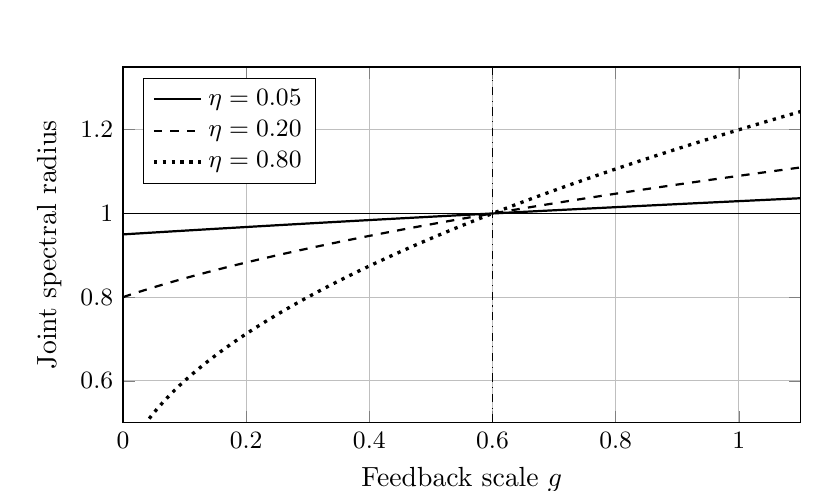
\begin{tikzpicture}
\begin{axis}[width=0.84\textwidth,height=6.1cm,
 xlabel={Feedback scale $g$},ylabel={Joint spectral radius},
 xmin=0,xmax=1.1,ymin=0.5,ymax=1.35,
 legend pos=north west,legend style={font=\small},
 tick label style={font=\small},grid=major]
\addplot[black,thick,domain=0:1.1,samples=120]
 {(0.4+1-0.05+sqrt((0.4-1+0.05)^2+4*x*0.05))/2};
\addlegendentry{$\eta=0.05$}
\addplot[black,dashed,thick,domain=0:1.1,samples=120]
 {(0.4+1-0.2+sqrt((0.4-1+0.2)^2+4*x*0.2))/2};
\addlegendentry{$\eta=0.20$}
\addplot[black,dotted,very thick,domain=0:1.1,samples=120]
 {(0.4+1-0.8+sqrt((0.4-1+0.8)^2+4*x*0.8))/2};
\addlegendentry{$\eta=0.80$}
\addplot[black,thin,forget plot] coordinates {(0,1)(1.1,1)};
\addplot[black,dashdotted,thin,forget plot] coordinates {(0.6,0.5)(0.6,1.35)};
\end{axis}
\end{tikzpicture}
\caption{Analytic illustration for $a=0.4$, $\kappa=1$. The three update rates share the boundary $g=0.6$ but yield different growth or decay rates. No AI models were trained to produce this figure.}
\label{fig:boundary}
\end{figure}

\section{Measurement and causal identification}
\label{sec:measurement}
\subsection{Machine autonomy exposure without arbitrary category scores}
Rather than assign unvalidated values such as $0.1$ to advisory software and $0.7$ to execution software, define a decision event and audit who had executable authority. For event $e$, let $v_e\geq0$ be a predeclared exposure weight and $d_e\in\{0,1\}$ indicate machine execution without a contemporaneous discretionary human approval. For a window $W$,
\begin{equation}
 \MAE_W=\frac{\sum_{e\in W}v_e d_e}{\sum_{e\in W}v_e}.
 \label{eq:mae}
\end{equation}
The denominator must be positive, and weights should represent comparable exposure, not arbitrary numbers of messages. Advisory use, order generation, execution authority, and online learning should be reported separately. Net exposure, gross executed exposure, and assets under management answer different questions and should not be mixed.

If authority is unobserved for some events, report an interval: the lower bound treats unknown events as nonautonomous and the upper bound treats them as autonomous. This makes missingness visible rather than assigning undocumented scores. It does not solve measurement error in $v_e$.

\subsection{Behavioral concentration is not provider concentration}
Provider concentration and common-cloud dependence are operational quantities. Behavioral concentration instead asks whether agents react along similar directions. Let $r_i\in\R^K$ be a nonzero response vector for agent $i$ on an independently designed panel of controlled perturbations, normalized to unit length after reporting its original response magnitude. With $w_i\geq0$ and $\sum_iw_i=1$, define
\begin{equation}
 S=\sum_i w_i r_i r_i^\top,\quad
 \ADC=\lambda_{\max}(S),\quad
 D_{\mathrm{eff}}=\frac{1}{\tr(S^2)}.
 \label{eq:adc}
\end{equation}
Here $\tr(S)=1$, so $\ADC$ is a directional-concentration descriptor. Zero-response agents require a separate reported mass; silently normalizing them is invalid. The perturbation panel, units, weights, and sampling variability all affect the estimate.

There is an important limitation. Two equal-weight agents with responses $r,r$ and two with responses $r,-r$ both yield the same $S$ and $\ADC=1$. Yet their aggregate signed responses are $r$ and zero, respectively. Thus \cref{eq:adc} cannot substitute for the signed aggregate response, price-impact direction, or the product $BC$. Diversity can remove reinforcing feedback, but it can also remove stabilizing behavior. There is no unconditional ``more diversity is safer'' theorem here.

\subsection{An identification impossibility without provenance}
\begin{proposition}[Observational equivalence of decision-maker labels]
\label{prop:identification}
Consider two economies with the same initial market-state distribution, the same market transition kernel conditional on aggregate actions, and the same conditional law of aggregate actions given every observable history. The economies can have different assignments of human and machine decision-maker labels. They nevertheless induce the same law for all observable market histories. No estimator using only those histories can consistently distinguish the two label assignments or identify different autonomy shares attached solely to those assignments.
\end{proposition}
\begin{proof}
The initial observable distributions coincide. If observable histories coincide in distribution through $t$, the assumed conditional action law and common market transition kernel imply the same distribution for the next observation. Induction establishes equality of all finite-dimensional observable distributions. Any statistic of those observations therefore has the same law in both economies; it cannot converge in probability to two distinct label-dependent constants.
\end{proof}
This is an application of ordinary observational equivalence, not a claim that financial attribution is impossible with richer data. Account-level decision provenance, randomly assigned architecture, authorized policy-update experiments, or credible external variation can break the equivalence. Historical prices alone do not reveal whether a self-exciting pattern was produced by humans, fixed algorithms, adaptive agents, or a mixture.

\subsection{Estimating the response system}
In a simulator with full state access, estimate $J$ by perturbing each normalized coordinate around a specified operating point and measuring the resulting joint next-state response. Use multiple perturbation sizes to test local linearity and independent random streams to quantify agent stochasticity. Finite differences of a mean response estimate a mean-map derivative, not a pathwise derivative of a discrete sampled action.

In observational data, fitting $z_{t+1}=Jz_t+e_{t+1}$ requires sufficient excitation, a defensible state representation, and restrictions controlling confounding and feedback-induced endogeneity. Hidden policy states typically require a state-space or input--output model. A reduced-form estimate may predict outcomes without identifying architecture-specific mechanisms; the paper must report which claim its design supports.

An uncertainty set $\mathcal J$ should reflect estimation uncertainty and relevant model misspecification. There is no distribution-free license to assign a narrow confidence interval to $\rho(J)$ by ignoring dependence, near-defective matrices, hidden states, or selected operating points. A claim of pre-crisis warning additionally requires lead time, false-alarm rates, and a prospectively fixed event definition.

\section{Intervention under uncertainty and liquidity feedback}
\label{sec:intervention}
A proposed intervention can reduce order size, slow an update, retain a previously approved policy, route a decision to review, or abstain from a specific action. These are not interchangeable. In particular, freezing learning need not cancel outstanding orders, and abstaining from new positions need not remove existing inventory risk.

\begin{proposition}[Common-norm robustness; standard sufficient condition]
\label{prop:robust}
Let $P\succ0$, $\norm{z}_P=(z^\top Pz)^{1/2}$, and let $\norm{J}_P$ be the associated induced norm. Suppose all admissible transition matrices satisfy $\norm{J}_P\leq\gamma<1$. For any sequence of those matrices and additive disturbances with $\norm{b_t}_P\leq\bar b$, the system $z_{t+1}=J_tz_t+b_t$ satisfies
\begin{equation}
 \norm{z_T}_P\leq\gamma^T\norm{z_0}_P+
 \bar b\frac{1-\gamma^T}{1-\gamma}.
 \label{eq:robustbound}
\end{equation}
A sufficient estimation-aware test is $\norm{\widehat J}_P+\epsilon\leq\gamma$ when $\norm{J-\widehat J}_P\leq\epsilon$ holds for every admissible $J$.
\end{proposition}
\begin{proof}
Submultiplicativity and the triangle inequality give $\norm{z_{t+1}}_P\leq\gamma\norm{z_t}_P+\bar b$. Iteration yields the geometric bound. The final sufficient test follows from $\norm{J}_P\leq\norm{\widehat J}_P+\norm{J-\widehat J}_P$.
\end{proof}
The common $P$ is essential: separate certificates with incompatible metrics do not certify arbitrary switching. A standard matrix formulation is $J^\top PJ\preceq\gamma^2P$ for every admissible matrix \citep{boyd1994}. In a nonlinear setting, analogous derivative bounds must hold throughout an invariant neighborhood; a certificate at one point is insufficient. A probabilistic estimation set yields only a guarantee conditional on its coverage event and assumptions.

\subsection{Why abstention is not automatically stabilizing}
Consider the scalar positive-feedback model with $a=0.4$, $\eta=0.2$, $\kappa=1$, and baseline $g_0=0.45$. Suppose an intervention retains a fraction $u$ of demand sensitivity but depth falls to a fraction $q(u)$ of baseline. The effective scale becomes
\begin{equation}
 g(u)=g_0\frac{u}{q(u)}.
 \label{eq:gatedepth}
\end{equation}
At $u=0.5$ and unchanged depth, $g=0.225$ and the model is more strongly stable. At $u=0.5$ and $q(u)=0.25$, $g=0.9$ and the model is unstable. These are constructed scenarios, not estimated liquidity elasticities. They show why evaluating abstention only through reduced individual trading ignores an essential equilibrium response.

Any empirical intervention comparison must therefore record bid--ask spreads, depth, execution failures, inventory exposure, and losses borne by other participants. An intervention that reduces one agent's losses by transferring risk or withdrawing market-making capacity is not automatically a system improvement. Operational deployment is outside this manuscript's scope.

\section{Executed numerical checks}
\label{sec:checks}
\subsection{Purpose and reproducibility}
The computations reported here test agreement between formulas and direct matrix calculations. They neither fit the model to a financial dataset nor train financial agents. \Cref{app:code} contains the exact self-contained Python/NumPy program used for the reported matrix checks. The run used NumPy 2.3.5, double-precision arrays, and seed 20260918 for the network samples. Last-digit differences across numerical libraries are immaterial to the stated tolerances.

\begin{table}[htbp]
\centering\small
\caption{Computed scalar-model examples. All rows use $a=0.4$ and $\kappa=1$. Parameters are illustrative and uncalibrated.}
\label{tab:scalar}
\begin{tabularx}{\textwidth}{Yrrrr}
\toprule
Case & $g$ & $\eta$ & $\rho(J_s)$ & $g\kappa/(1-a)$\\
\midrule
Stable feedback & 0.300 & 0.20 & 0.916228 & 0.500\\
Boundary & 0.600 & 0.20 & 1.000000 & 1.000\\
Unstable feedback & 0.900 & 0.20 & 1.069042 & 1.500\\
Same unstable gain, slower learning & 0.900 & 0.05 & 1.022311 & 1.500\\
Same unstable gain, faster learning & 0.900 & 0.80 & 1.154400 & 1.500\\
Baseline before action gate & 0.450 & 0.20 & 0.960555 & 0.750\\
Gate with depth unchanged & 0.225 & 0.20 & 0.891548 & 0.375\\
Gate with depth at one quarter & 0.900 & 0.20 & 1.069042 & 1.500\\
\bottomrule
\end{tabularx}
\end{table}

\subsection{Verification results}
The scalar Cartesian grid comprises five values each of $a$, $\eta$, $g$, and $\kappa$, giving $5^4=625$ cases away from the boundary. All direct eigenvalue classifications agree with $g\kappa<1-a$. The largest absolute difference between the formula and direct eigenvalue calculations is approximately $2.22\times10^{-16}$.

The network check uses 250 independently generated nonnegative pairs with $d=3$ market coordinates and $n=4$ adaptive states, along with randomized admissible scalar parameters. All classifications agree with \cref{eq:boundary}; the largest formula discrepancy is approximately $2.89\times10^{-15}$. These are numerical consistency tests, not 250 independent market experiments and not evidence of generalization to large language models.

The program also verifies the switching example, the transient-amplification example, and the signed-response concentration counterexample. The switching product has spectral radius $4.486068$, corresponding to an asymptotic per-step factor of approximately $2.118034$ under periodic alternation. The stable nonnormal example reaches the previously reported gain $8.212429$. Both identical and opposite response panels have $\ADC=1$, despite different aggregate signed responses.

The mathematical proofs, not the finite grid, justify the universal statements within the specified model. The computations provide an implementation check and reproducible illustrations. No confidence interval or significance claim is attached to an exact algebra check.

\section{Prospective multi-agent experimental protocol}
\label{sec:experiments}
\textbf{Status: not executed.} This section specifies the experiment needed to test whether the model quantities have useful meaning in richer financial environments. It must be registered or otherwise frozen before inspecting confirmatory outcomes.

\subsection{Research hypotheses and their rejection conditions}
\begin{table}[htbp]
\centering\small
\caption{Prospective hypotheses. No row is reported as an established empirical finding.}
\label{tab:hypotheses}
\begin{tabularx}{\textwidth}{p{0.07\textwidth}YY}
\toprule
ID & Hypothesis & Evidence against the proposed claim \\
\midrule
H1 & A joint response estimate predicts stress amplification beyond ordinary market covariates. & No reproducible incremental prediction on held-out regimes.\\
H2 & Matching measured feedback reduces architecture-specific outcome differences. & Large architecture effects remain after reliable response matching.\\
H3 & Increased reinforcing response alignment increases loss amplification in the specified environment. & Effects disappear under matched depth and exposures, or reverse outside selected cells.\\
H4 & An uncertainty-aware gate improves a predeclared loss--liquidity trade-off. & Apparent benefits rely on disappearing liquidity, oracle information, or shifted losses.\\
H5 & A boundary estimated in one agent family transfers to a held-out family or simulator. & Transfer requires unrestricted refitting or yields unacceptable uncertainty.\\
\bottomrule
\end{tabularx}
\end{table}
The ``calm but fragile'' hypothesis is secondary. It requires jointly measuring ordinary variation and losses under a separately specified shock distribution. A lower volatility statistic coupled with a higher local spectral radius is not itself a measured increase in tail losses.

\subsection{Environment and economic accounting}
The first market should contain an exchange, finite cash and inventory balances, explicitly funded positions, and a price-formation mechanism. Every fill transfers inventory and cash between counterparties, with fees and external cash flows separately accounted for. The simulator must reject unfunded or otherwise infeasible actions according to the declared rules. In a leveraged extension, margin calculations and forced liquidation must be implemented and audited.

If public historical order-flow or price data are used for calibration, separate periods for calibration, validation, and stress evaluation are required. Matching a handful of stylized facts is a useful diagnostic but does not prove that a simulator captures crisis mechanisms. Price replays without endogenous market impact cannot test the central feedback hypothesis: the agents must be able to change subsequent market states.

ABIDES is a candidate infrastructure described in prior work \citep{byrd2019}; the selected implementation, version, matching rules, and modifications must be recorded. An independent second simulator should use a materially different implementation while preserving the experimental economic contract.

\subsection{Agent families and matched baselines}
A minimum design should compare adaptive expectation rules, a simple value-learning agent, a more expressive learning policy, and an inference-only language-model policy. Optional online adaptation for an LLM must be operationally defined: weights, external memory, retrieved examples, prompts, or tool policies may update differently. Merely calling an LLM repeatedly is not evidence of online parameter learning.

Each adaptive policy needs a paired baseline with the same architecture, information, constraints, and checkpoint, but the relevant adaptation channel disabled during evaluation. Additional baselines should include nonadaptive rule-based agents, ordinary risk-control feedback, and adaptive expectation agents not described as AI. A human-like rule is not a human-subject benchmark. A claim about replacing human decisions eventually requires actual human evidence or a validated behavioral model with stated limits.

Differences in capital, risk tolerance, signal quality, latency, execution permissions, and available computation should be held fixed where possible and explicitly decomposed where impossible. A language model with richer information and a longer decision budget is not a clean architecture-only comparison with a small tabular learner.

\subsection{Factor design and compute discipline}
Begin with a small mechanism-identification pilot. A proposed affordable pilot crosses three participation levels, three response-sharing conditions, three update schedules, and two depth regimes: $3\times3\times3\times2=54$ cells. Ten independent market seeds per cell would require 540 trajectories per paired policy condition. These are planning choices, not a power calculation or completed run count.

Use the pilot only to identify implementation failures, estimate variance, and choose financially meaningful outcome scales. Confirmatory seeds, shock paths, and held-out architectures must then be fresh. A proposed second stage expands only the dimensions needed to distinguish competing mechanisms. A large six-dimensional grid or 10,000-agent population should not precede basic accounting validation and estimator recovery.

Avoid treating thousands of ticks within one market run as independent replications. The independent unit is generally the market episode or another justified cluster. Paired shock paths can improve precision, but they do not remove dependence within episodes or make different agents in the same market independent samples.

\subsection{Shock families and timing}
Predeclare shocks to fundamentals, depth, funding requirements, information quality, update synchronization, and decision-service availability. Apply information-corruption scenarios only inside an isolated, authorized simulation. A shared model change should be tested both synchronously and asynchronously, and compared with an equally large change to a non-AI policy.

Hold shock realizations paired across treatment and baseline where the comparison requires identical external conditions. Randomize shock timing within a predeclared range to reduce phase-specific artifacts. Stress amplitudes must be reported in economically interpretable units as well as normalized model units. There is no presumption that one calendar-time horizon applies to both an exchange and a fund-redemption environment.

\subsection{Primary outcomes and statistical analysis}
For a price-forming environment, a useful primary outcome is a predeclared, horizon-limited cumulative price dislocation from a simulated fundamental reference, normalized by the scale of the initiating shock. Report the unnormalized numerator and denominator, and avoid ratios near a zero denominator. In an empirical market, the fundamental reference is not observed directly and requires a separate identification argument.

Secondary outcomes should include liquidation losses, execution shortfall, spread, depth, order imbalance, inventory concentration, and recovery time. Distributional tail loss is meaningful only after defining whose loss is measured and over what shock distribution. Mark-to-market wealth transfers should not be mislabeled aggregate social losses. Deadweight liquidation costs, default shortfalls, and real-economy outcomes are distinct quantities.

Compare a baseline predictor using volatility, depth, spreads, leverage, and ordinary order-flow statistics with an augmented predictor that also uses the proposed feedback variables. Evaluate temporal and architecture-held-out prediction with uncertainty, calibration, and economic effect sizes. If the outcome is a distress event, report lead time and false alarms rather than only an area-under-curve statistic. Thresholds and model-selection rules must be fixed without access to the held-out outcomes.

Use cluster-aware uncertainty estimates or independent-run resampling, declare the multiple-testing family, and report failed and null conditions. A practical power analysis should use pilot variance and a justified smallest effect of interest, not a universal ``30 seeds'' rule.

\subsection{Boundary estimation and terminology}
A sharp-looking heatmap is not proof of a phase transition. First test whether a continuous, nonlinear, or threshold model better describes held-out outcomes. Distinguish a local eigenvalue crossing from a finite-sample increase in crisis frequency and from a true large-population phase transition. A statistical-physics claim would require an appropriate limiting sequence, scaling analysis, and finite-size evidence.

Report a region of uncertainty around any fitted boundary. When the estimator cannot distinguish stable and unstable mechanisms under realistic observation noise, that limitation is a result. A model-conditioned warning that is frequently indeterminate may still be scientifically useful, but it should not be marketed as a universal instability detector.

\section{Prospective empirical validation}
\label{sec:empirical}
\textbf{Status: not executed; no partner access is claimed.} The crucial bottleneck is observation of decision provenance and adaptation, not simply downloading more price histories. An empirical dataset would ideally record anonymized decision or account identifiers, timestamps, execution authority, policy versions, update timing, exposure limits, and market outcomes. Such records require lawful access, institutional cooperation, and appropriate privacy controls.

A partner-assisted study could exploit an authorized staggered rollout or a preplanned randomized change to update scheduling, provided risk controls and research oversight permit it. A model-provider outage or update is not automatically exogenous: exposure may differ systematically across institutions, and the event may coincide with other market information. A difference-in-differences or event-study label does not remove those problems. The identification argument must specify the assignment mechanism, comparison group, anticipation, spillovers, and relevant confounders.

An initial empirical contribution could be measurement validation rather than crisis forecasting. For example, compare response estimates obtained from controlled internal replay or paper trading with responses around authorized small operational changes. Test whether provider labels predict actual signed behavioral similarity, and whether policy update logs distinguish learning from ordinary signal refresh. These questions can reveal whether the proposed state variables are observable enough to support the larger program.

Shadow evaluation permits predictions and alerts to be recorded without authorizing trades. It is a possible stage before intervention research, not a substitute for causal validation. Predictions must be timestamped and evaluated against later outcomes under frozen scoring rules. Where access is unavailable, the paper should remain a simulation or theoretical contribution and restrict its conclusions accordingly.

Cross-domain extension requires separate validation. A limit-order-book price perturbation is not the same object as a depositor's redemption incentive or a lender's credit supply response. A genuine unifying contribution would show which state transformations and feedback quantities remain meaningful across those settings, where the mapping fails, and what institutional variables cannot be abstracted away.

\section{Limitations, responsible use, and wider significance}
\label{sec:limits}
\subsection{Scientific limitations}
The tractable model uses a common first-order learning rate, a fixed reference point, and nonnegative response matrices. It omits endogenous innovation in strategies, strategic deception, discontinuous liquidation rules, endogenous entry and exit, and general-equilibrium wealth effects. Its spectral boundary is neither an asset-pricing theorem nor a universal condition for crises. Some instability modes may be damped by limits, while finite disturbances can cause defaults even around a locally stable equilibrium.

The complete joint state may be inaccessible for modern agents. Hidden memory, discrete version changes, stochastic sampling, and proprietary risk overlays can undermine smooth finite-dimensional approximations. Estimated feedback may be highly uncertain exactly where extreme events matter. Identifying a persistent empirical feedback coefficient does not identify an economically optimal intervention.

The present numerical checks are intentionally small and uncalibrated. They provide no evidence of a global machine-participation threshold, real-market prediction, architecture-independent transfer, or the superiority of an abstention system. They also do not establish a new scientific paradigm. Any submission must communicate this evidence boundary in the abstract as well as the methods.

\subsection{Research ethics and operational boundaries}
All agent-interaction and information-corruption experiments should remain in controlled environments unless separately authorized. No experiment proposed here requires placing deceptive orders, manipulating public markets, or using customer data without permission. Human-subject work and sensitive institution-level records require relevant review, consent or lawful basis, data minimization, and secure handling.

Publication should document model versions, datasets, licenses, prompts that may legally be shared, code changes, and observed failure modes. Public generated explanations may be studied as outputs, but should not be treated as verified internal reasoning or a causal account of an agent's decision. No claim depends on access to private model reasoning.

\subsection{What would make the contribution globally useful}
The potential value is a measurement and validation framework that helps institutions understand interactions among decision systems, rather than another predictor of asset prices. To support wider use, the framework would need reliable estimation from realistic observations, added value over existing risk measures, transfer across relevant architectures and institutions, and evidence about intervention costs and spillovers. The FSB's monitoring work and its 2026 consultation on responsible adoption provide institutional context for such questions, not endorsement of this manuscript \citep{fsb2025,fsb2026}.

A globally relevant result need not claim that all financial laws have changed. A precisely demonstrated failure of an existing diagnostic, together with a better measurable replacement and clearly delimited applicability, could materially advance the field. Conversely, evidence that conventional feedback and liquidity models already explain the alleged machine transition would be an important correction to exaggerated claims.

\section{Conclusion}
The defensible question is not whether financial markets cease to obey all familiar principles when AI becomes prevalent. It is whether adaptive delegation changes economically measurable feedback in ways that existing diagnostics fail to capture. The correct local state includes both the market and its learning participants. Under a restricted positive-feedback specialization, the stability boundary depends on market persistence and the network's loop gain, while learning speed changes dynamics without necessarily moving the boundary. Counterexamples show why frozen eigenvalues, normal-period volatility, provider diversity, and individual abstention are insufficient certificates of financial safety.

The next scientific step is empirical in the broad sense: recover these quantities in a validated simulator, show incremental and transferable prediction, identify causal effects, and then test observational feasibility with appropriate real-world data. The complete manuscript provides a foundation and an auditable plan. A paradigm-forming contribution would require successful evidence at those stages, theoretical novelty beyond standard tools, and independent uptake; those outcomes cannot be manufactured by an ambitious title or a longer paper.

\section*{Data, code, and disclosure statement}
No financial dataset, human-subject dataset, or proprietary institutional record was used to produce the current results. Numerical findings in \cref{sec:checks} come from the program reproduced in \cref{app:code}. All proposed market experiments remain unexecuted. The manuscript was developed with AI assistance from a supplied concept note; prospective named authors must independently verify its mathematics, sources, and claims and take responsibility for the final submission. No author identity, institutional affiliation, funding award, ethics approval, data partnership, or external endorsement is asserted here.

\clearpage
\begingroup
\small
\setlength{\bibsep}{4pt}
\begin{thebibliography}{99}
\bibitem[Arthur et~al.(1996)]{arthur1996}
W. Brian Arthur, John H. Holland, Blake LeBaron, Richard Palmer, and Paul Tayler.
\newblock Asset Pricing Under Endogenous Expectations in an Artificial Stock Market.
\newblock Santa Fe Institute Working Paper 96-12-093, 1996.
\newblock \url{https://www.santafe.edu/research/results/working-papers/asset-pricing-under-endogenous-expectations-in-an-}.

\bibitem[Brock and Hommes(1998)]{brock1998}
William A. Brock and Cars H. Hommes.
\newblock Heterogeneous beliefs and routes to chaos in a simple asset pricing model.
\newblock \emph{Journal of Economic Dynamics and Control}, 22(8--9):1235--1274, 1998.
\newblock \url{https://doi.org/10.1016/S0165-1889(98)00011-6}.

\bibitem[Brunnermeier and Pedersen(2009)]{brunnermeier2009}
Markus K. Brunnermeier and Lasse Heje Pedersen.
\newblock Market Liquidity and Funding Liquidity.
\newblock \emph{The Review of Financial Studies}, 22(6):2201--2238, 2009.
\newblock \url{https://doi.org/10.1093/rfs/hhn098}.

\bibitem[Calvano et~al.(2020)]{calvano2020}
Emilio Calvano, Giacomo Calzolari, Vincenzo Denicol\`o, and Sergio Pastorello.
\newblock Artificial Intelligence, Algorithmic Pricing, and Collusion.
\newblock \emph{American Economic Review}, 110(10):3267--3297, 2020.
\newblock \url{https://doi.org/10.1257/aer.20190623}.

\bibitem[Perdomo et~al.(2020)]{perdomo2020}
Juan C. Perdomo, Tijana Zrnic, Celestine Mendler-D\"unner, and Moritz Hardt.
\newblock Performative Prediction.
\newblock \emph{Proceedings of Machine Learning Research}, 119:7599--7609, 2020.
\newblock \url{https://proceedings.mlr.press/v119/perdomo20a.html}.

\bibitem[Narang et~al.(2023)]{narang2023}
Adhyyan Narang, Evan Faulkner, Dmitriy Drusvyatskiy, Maryam Fazel, and Lillian J. Ratliff.
\newblock Multiplayer Performative Prediction: Learning in Decision-Dependent Games.
\newblock \emph{Journal of Machine Learning Research}, 24(202):1--56, 2023.
\newblock \url{https://jmlr.org/papers/v24/22-0131.html}.

\bibitem[Farina and Perdomo(2026)]{farina2026}
Gabriele Farina and Juan Carlos Perdomo.
\newblock The Stability of Online Algorithms in Performative Prediction.
\newblock arXiv:2602.24207v2, 3 June 2026. Preprint.
\newblock \url{https://arxiv.org/abs/2602.24207v2}.

\bibitem[Anand et~al.(2026)]{anand2026}
Kartik Anand, Sophia Kazinnik, Agnese Leonello, and Ettore Panetti.
\newblock Ex Machina: financial stability in the age of artificial intelligence.
\newblock European Central Bank Working Paper Series, No. 3225, 2026.
\newblock \url{https://doi.org/10.2866/4103076}.

\bibitem[Colliard et~al.(2026)]{colliard2026}
Jean-Edouard Colliard, Thierry Foucault, and Stefano Lovo.
\newblock Algorithmic Pricing and Liquidity in Securities Markets.
\newblock \emph{The Review of Financial Studies}, hhag010, 2026.
\newblock \url{https://doi.org/10.1093/rfs/hhag010}.

\bibitem[Financial Stability Board(2024)]{fsb2024}
Financial Stability Board.
\newblock The Financial Stability Implications of Artificial Intelligence.
\newblock 14 November 2024.
\newblock \url{https://www.fsb.org/uploads/P14112024.pdf}.

\bibitem[Financial Stability Board(2025)]{fsb2025}
Financial Stability Board.
\newblock Monitoring Adoption of Artificial Intelligence and Related Vulnerabilities in the Financial Sector.
\newblock 10 October 2025.
\newblock \url{https://www.fsb.org/2025/10/monitoring-adoption-of-artificial-intelligence-and-related-vulnerabilities-in-the-financial-sector/}.

\bibitem[Financial Stability Board(2026)]{fsb2026}
Financial Stability Board.
\newblock Sound Practices for Responsible Adoption of Artificial Intelligence (AI): Consultation report.
\newblock 10 June 2026. This reference identifies the consultation version, not a legal requirement.
\newblock \url{https://www.fsb.org/2026/06/sound-practices-for-responsible-adoption-of-artificial-intelligence-ai-consultation-report/}.

\bibitem[Boyd et~al.(1994)]{boyd1994}
Stephen Boyd, Laurent El Ghaoui, Eric Feron, and Venkataramanan Balakrishnan.
\newblock \emph{Linear Matrix Inequalities in System and Control Theory}.
\newblock SIAM, 1994.
\newblock \url{https://web.stanford.edu/~boyd/lmibook/}.

\bibitem[Khalil(2002)]{khalil2002}
Hassan K. Khalil.
\newblock \emph{Nonlinear Systems}. Third edition.
\newblock Prentice Hall, 2002.
\newblock \url{https://www.egr.msu.edu/~khalil/NonlinearSystems/}.

\bibitem[Byrd et~al.(2019)]{byrd2019}
David Byrd, Maria Hybinette, and Tucker Hybinette Balch.
\newblock ABIDES: Towards High-Fidelity Market Simulation for AI Research.
\newblock arXiv:1904.12066, 2019. This reference identifies the preprint version.
\newblock \url{https://arxiv.org/abs/1904.12066}.
\end{thebibliography}
\endgroup

\clearpage
\appendix
\section{Proofs and technical qualifications}
\label{app:proofs}
\subsection{Local stability and the limits of linearization}
For the stable part of Proposition~\ref{prop:local}, choose $\gamma\in(\rho(J^*),1)$. Finite-dimensional matrix theory provides an equivalent vector norm with $\norm{J^*}<\gamma$. Continuity of $D\Phi$ provides a convex neighborhood of $z^*$ and $\widetilde\gamma<1$ such that $\norm{D\Phi(z)}\leq\widetilde\gamma$ throughout that neighborhood. The mean-value integral yields
\begin{equation}
 \norm{\Phi(z)-z^*}\leq\widetilde\gamma\norm{z-z^*}.
\end{equation}
A sufficiently small norm ball is invariant; iteration gives exponential decay. The unstable part is the standard discrete-time linearization instability result: a derivative eigenvalue outside the closed unit disk produces a locally expanding direction and rules out Lyapunov stability for a continuously differentiable map. No conclusion is asserted from an eigenvalue on the unit circle alone. The result concerns the fixed autonomous map and its fixed point, not an arbitrary sequence of re-estimated Jacobians.

\subsection{Proof of the positive-feedback boundary}
\label{app:positiveproof}
Let $\nu=\rho(BC)$ and define
\begin{equation}
 r_+=\frac{a+1-\eta+\sqrt{(a-1+\eta)^2+4g\eta\nu}}{2}.
\end{equation}
When $g\nu>0$, Perron--Frobenius theory supplies $v\geq0$, $v\ne0$, with $BCv=\nu v$. Then $Cv\ne0$ and
\begin{equation}
 w=\frac{\eta}{r_+-1+\eta}Cv
\end{equation}
satisfies $J_+(v,w)^\top=r_+(v,w)^\top$. Hence $r_+$ is an eigenvalue.

To show that no eigenvalue has greater modulus, let $(v,w)$ be a nonzero eigenvector with eigenvalue $\lambda$. Eigenvalues equal to $a$ or $1-\eta$ have modulus at most $r_+$. For the others, eliminating $w$ gives
\begin{equation}
 BCv=\frac{(\lambda-a)(\lambda-1+\eta)}{g\eta}v.
\end{equation}
If $|\lambda|>r_+$, then $|\lambda|>\max(a,1-\eta)$ and
\begin{align}
 |(\lambda-a)(\lambda-1+\eta)|
 &\geq(|\lambda|-a)(|\lambda|-(1-\eta))\\
 &>(r_+-a)(r_+-(1-\eta))=g\eta\nu.
\end{align}
This contradicts the spectral-radius bound on eigenvalues of $BC$. Thus $\rho(J_+)=r_+$. If $g=0$, the matrix is block triangular. If $\nu=0$ and $g>0$, the same elimination excludes every eigenvalue outside $\{a,1-\eta\}$, so the formula reduces to $\max(a,1-\eta)$ and remains valid.

Finally, $r_+<1$ is equivalent to
\begin{equation}
 \sqrt{(a-1+\eta)^2+4g\eta\nu}<1-a+\eta.
\end{equation}
The right side is positive. Squaring and simplifying yields $g\nu<1-a$ because $\eta>0$. Equality and strict reversal follow identically. For a finite-dimensional constant linear system, all eigenvalues inside the unit disk are equivalent to asymptotic stability. This proves \cref{thm:positive}.

\subsection{What the boundary does not imply}
A positive real eigenvalue passing through one identifies loss of local linear stability in the specified model. It does not determine the nonlinear attractor, whether prices crash or grow, whether an institution defaults, or whether a finite disturbance remains inside the modeled region. A nonlinear extension could saturate or switch into another regime. An observed financial crisis can also occur without this crossing, for example when an external shock overwhelms solvency buffers.

The result uses a single persistence scalar $a$ and a common $\eta$. Allowing asset-specific persistence, asymmetric learning rates, delayed observation, or signed response matrices removes the simple formula unless further structure is proved. A claimed universal surface in six aggregate variables would need to show that the omitted state is either irrelevant, bounded, or measured. The current theorem does not establish such sufficiency.

\subsection{Stochastic and nonlinear robustness}
For a nonlinear map $\Phi_t$ with a common reference point, suppose the induced $P$-norm of every derivative on a convex ball of radius $r$ is at most $\gamma<1$. Then the same Lipschitz argument yields the disturbance bound in \cref{eq:robustbound}. If $\bar b\leq(1-\gamma)r$ and the initial state is inside the ball, that ball is invariant. With an evolving reference point, its motion must appear as an additional disturbance; ignoring that drift changes the claim.

If an estimated uncertainty set covers the actual matrices with probability at least $1-\delta$ over the relevant horizon, the robust bound holds on that coverage event. Marginal per-time coverage does not automatically imply simultaneous horizon coverage. Model updates, adaptive sampling, and post-selection can invalidate a naive confidence statement. These statistical issues are work remaining, not solved by the deterministic norm inequality.

\section{Executable reproduction of the numerical checks}
\label{app:code}
Copy the following listing into \texttt{verify\_math.py} and run it with Python 3 and NumPy. The program has no network access, downloads no financial data, and trains no models. All numerical parameters and random seeds are explicit. It prints the values reported in \cref{sec:checks} and stops with an assertion error if an algebraic check fails.
\begin{lstlisting}
"""Deterministic algebra checks for the Machine Markets working paper.
These are NOT calibrated markets, agent experiments, or empirical evidence.
Requires Python 3 and NumPy. Run: python verify_math.py
"""
import json
import numpy as np


def spectral_radius(matrix):
    matrix = np.asarray(matrix, dtype=float)
    if matrix.ndim != 2 or matrix.shape[0] != matrix.shape[1]:
        raise ValueError("Expected a square matrix")
    if not np.isfinite(matrix).all():
        raise ValueError("Nonfinite matrix entry")
    return float(np.max(np.abs(np.linalg.eigvals(matrix))))


def scalar_matrix(a, g, eta, kappa=1.0):
    if not (0 <= a < 1 and 0 < eta <= 1 and g >= 0 and kappa >= 0):
        raise ValueError("Parameters violate the proposition assumptions")
    return np.array([[a, g], [eta * kappa, 1 - eta]])


def rho_formula(a, g, eta, kappa=1.0):
    return float((a + 1 - eta + np.sqrt((a - 1 + eta)**2
                 + 4 * g * eta * kappa)) / 2)


def main():
    rows = []
    for label, g, eta in [
        ("stable feedback", 0.30, 0.20),
        ("boundary", 0.60, 0.20),
        ("unstable feedback", 0.90, 0.20),
        ("same unstable gain, slower learning", 0.90, 0.05),
        ("same unstable gain, faster learning", 0.90, 0.80),
        ("baseline before action gate", 0.45, 0.20),
        ("gate, depth unchanged", 0.225, 0.20),
        ("gate, depth reduced to one quarter", 0.90, 0.20),
    ]:
        radius = spectral_radius(scalar_matrix(0.4, g, eta))
        assert abs(radius - rho_formula(0.4, g, eta)) < 1e-12
        rows.append(dict(case=label, a=0.4, g=g, eta=eta, kappa=1.0,
                         radius=radius))

    # A deterministic Cartesian grid, not a Monte Carlo experiment.
    scalar_checks = 0
    max_error = 0.0
    for a in [0.1, 0.3, 0.5, 0.7, 0.9]:
        for eta in [0.05, 0.2, 0.5, 0.8, 1.0]:
            for g in [0.07, 0.17, 0.37, 0.67, 1.07]:
                for kappa in [0.15, 0.45, 0.85, 1.25, 1.75]:
                    radius = spectral_radius(scalar_matrix(a, g, eta, kappa))
                    max_error = max(max_error,
                        abs(radius - rho_formula(a, g, eta, kappa)))
                    assert abs(g * kappa - (1 - a)) > 1e-8
                    assert (radius < 1) == (g * kappa < 1 - a)
                    scalar_checks += 1

    # Independent network formula checks with a fixed seed.
    rng = np.random.default_rng(20260918)
    network_checks = 0
    max_network_error = 0.0
    for _ in range(250):
        d, n = 3, 4
        B = rng.uniform(0, 1, (d, n)) / n
        C = rng.uniform(0, 1, (n, d)) / d
        a = float(rng.uniform(0.05, 0.95))
        eta = float(rng.uniform(0.05, 1.0))
        g = float(rng.uniform(0.01, 4.0))
        J = np.block([[a*np.eye(d), g*B],
                      [eta*C, (1-eta)*np.eye(n)]])
        nu = spectral_radius(B @ C)
        radius = spectral_radius(J)
        pred = rho_formula(a, g, eta, nu)
        max_network_error = max(max_network_error, abs(radius - pred))
        assert abs(radius - pred) < 1e-10
        assert abs(g*nu - (1-a)) > 1e-8
        assert (radius < 1) == (g*nu < 1-a)
        network_checks += 1

    # Frozen eigenvalues do not certify an arbitrarily switched system.
    J1 = np.array([[0.5, 2.0], [0.0, 0.5]])
    J2 = J1.T
    switch_radius = spectral_radius(J2 @ J1)
    assert spectral_radius(J1) == 0.5
    assert spectral_radius(J2) == 0.5
    assert switch_radius > 1

    # Stable eigenvalues can coexist with large finite-horizon gain.
    J = np.array([[0.8, 4.0], [0.0, 0.8]])
    gains = [float(np.linalg.norm(np.linalg.matrix_power(J, h), 2))
             for h in range(51)]
    peak_h = int(np.argmax(gains))
    assert spectral_radius(J) < 1 and max(gains) > 8

    # A Gram concentration score loses the direction of action alignment.
    r = np.array([1.0, 0.0])
    same = np.stack([r, r])
    opposite = np.stack([r, -r])
    def adc(R):
        return float(np.linalg.eigvalsh(R.T @ R / len(R))[-1])
    assert adc(same) == adc(opposite) == 1.0
    assert np.linalg.norm(same.mean(axis=0)) == 1.0
    assert np.linalg.norm(opposite.mean(axis=0)) == 0.0

    out = dict(scalar_cases=rows, scalar_grid_checks=scalar_checks,
               max_scalar_formula_error=max_error,
               network_checks=network_checks,
               max_network_formula_error=max_network_error,
               switching_product_radius=switch_radius,
               switching_per_step_growth=np.sqrt(switch_radius),
               nonnormal_radius=0.8, nonnormal_peak_h=peak_h,
               nonnormal_peak_gain=max(gains),
               concentration_same=adc(same),
               concentration_opposite=adc(opposite),
               numpy_version=np.__version__)
    print(json.dumps(out, indent=2))

if __name__ == "__main__":
    main()
\end{lstlisting}

\clearpage
\section{Source provenance and revisions to the supplied concept note}
\label{app:provenance}
The user-supplied document \emph{Pasted markdown.md} is the conceptual basis of this manuscript. It proposes the title, the market--learning feedback question, six organizing dimensions, critical-regime analysis, and a long-term ambition extending beyond trading. It is a planning document, not an empirical source. The table below explicitly separates retained framing from changes introduced during drafting and literature verification.

\begin{longtable}{p{0.28\textwidth}p{0.66\textwidth}}
\caption{Transparent changes from the concept note.}\label{tab:provenance}\\
\toprule
Concept-note element & Treatment in this manuscript \\
\midrule
\endfirsthead
\toprule Concept-note element & Treatment in this manuscript \\
\midrule
\endhead
\bottomrule
\endfoot
Human-to-machine market transition & Retained as the motivating question; no assertion that accounting or all classical finance becomes invalid.\\
Joint evolution of market and policy & Retained, while explicitly acknowledging adaptive-expectations and performative-prediction precedents.\\
Partial feedback product & Replaced by the full augmented Jacobian, including direct persistence and policy-state dynamics.\\
Machine-market criticality & Retained as a descriptive local label; supplemented with transient gains, time-varying products, and robustness qualifications.\\
Arbitrary autonomy scores & Replaced by event-level execution-authority measurement, exposure weights, and missingness bounds.\\
Weighted concentration index & Replaced by an explicit response-panel descriptor plus a counterexample showing why concentration alone is insufficient.\\
Candidate ``laws'' & Reclassified as hypotheses or model-conditioned results. Update speed and volatility receive explicit counterexamples to universal claims.\\
Universal AI participation threshold & Replaced by a conditional surface in a solvable positive-feedback model; no universal percentage is claimed.\\
Act/freeze/abstain safety idea & Retained as a prospective comparison; liquidity withdrawal and remaining inventory risk are modeled as possible failure channels.\\
Large multi-agent experiment & Specified as future work, beginning with a small validation pilot. No fabricated agent outcomes are inserted.\\
2025--2026 source links & Only independently checked primary-source references used in the text were retained. Other concept-note links are not treated as established evidence here.\\
Paradigm-level ambition & Retained as an eventual evidence standard, not as a current quality rating or promised outcome.\\
\end{longtable}
The mathematical examples and executed matrix checks were developed for this draft and were not reported findings in the concept note. The 2026 ECB working paper is cited by its verified working-paper version; the surrounding Research Bulletin uses an earlier-year citation to its predecessor. The present reference deliberately identifies the version consulted rather than silently combining versions.

\clearpage
\section{Evidence contract for a completed flagship paper}
\label{app:contract}
A final empirical manuscript should replace the prospective sections only when the corresponding evidence exists. The following is an acceptance contract for the research program, not a list of results already achieved.

\paragraph{Theoretical increment.}
Identify and defend at least one result that is not merely a standard local-stability theorem under new names. Possible targets include partial-observation identification bounds, statistically valid finite-horizon certificates under endogenous adaptation, or a causal decomposition that separates adaptive-policy feedback from ordinary liquidity feedback. The choice should follow a nearest-neighbor literature review.

\paragraph{Mechanism evidence.}
Recover known parameters in a synthetic system before interpreting estimates from a market simulator. Then show that interventions on the proposed feedback channel, with capital, information, and market design controlled, change the specified financial outcome as predicted. Include alternative explanations and conditions in which the hypothesis fails.

\paragraph{Predictive and economic relevance.}
Demonstrate added value beyond conventional observables on genuinely held-out conditions. Report uncertainty, false alarms, lead time, and financially meaningful effect sizes. Do not select the only successful architecture, asset, shock, or seed after seeing results.

\paragraph{Transfer and falsification.}
Test a held-out agent family and an independently implemented environment. Map failure regions. A second financial domain is desirable for a broad framework, but not permission to weaken the first domain's identification. Universal laws require much more than success on two datasets.

\paragraph{Responsible intervention evidence.}
Evaluate feasible interventions using only information available at the decision time. Include liquidity, execution costs, inventory exposure, externalities, and the conditions under which a proposed gate cannot certify anything. An oracle controller is a diagnostic upper benchmark, not a deployable competitor.

\paragraph{External validation and independent reproduction.}
Establish whether the quantities can be measured with realistic institutional data, or delimit the work to simulation. Release reproducible materials where permitted, obtain independent verification, and distinguish peer-reviewed acceptance from subsequent scientific adoption. Community use and durable explanatory power, not a preassigned score, determine whether a contribution becomes paradigm forming.

\paragraph{Completion statement.}
This version completes the document structure, derivations, source-backed framing, numerical algebra checks, and experimental specification. It does not complete the scientific program. The companion Word roadmap translates the acceptance contract into concrete tasks, dependencies, outputs, and review gates.
\end{document}
